\section{Resultados e Discussão}

A Tabela~\ref{tab:principal} traz o resultado de cada instância e da programação dinâmica; a Tabela~\ref{tab:bb} traz o comportamento do Branch-and-Bound em 15 minutos; as Figuras~\ref{fig:razao} e~\ref{fig:tempos} resumem a qualidade e o tempo. Todos os números vêm de \texttt{resultados\_longos/resultados.csv}, e em toda instância em que os dois algoritmos terminaram os valores coincidiram.

\begin{table}[ht]\centering\footnotesize\setlength{\tabcolsep}{4pt}
\caption{Resultados nas 12 instâncias. Ótimo/melhor: ótimo provado (sem marca) ou melhor valor encontrado, sem prova de otimalidade ($^*$). Heur.: heurística do Trabalho~1. Razão: Heur./ótimo. DP: largura $w$, tempo e memória estimada; ``---'' indica programação dinâmica inviável ($w>26$).}\label{tab:principal}
\begin{tabular}{lrrrrcrrr}\hline
Instância & $n$ & $m$ & Ótimo/melhor & Heur. & Razão & $w$ & DP (s) & Mem. (MB) \\\hline
01\_ALE\_n100 & 100 & 200 & 168 & 158 & 0{,}940 & 21 & 0{,}173 & 26 \\
02\_ALE\_n120 & 120 & 240 & 204 & 196 & 0{,}961 & 26 & 5{,}139 & 845 \\
03\_PM1\_n120 & 120 & 240 & 83 & 69 & 0{,}831 & 26 & 5{,}147 & 845 \\
04\_TORO\_8x250 & 2000 & 4000 & 1406 & 1114 & 0{,}792 & 17 & 0{,}811 & 16 \\
05\_TORO\_10x200 & 2000 & 4000 & 1386 & 1080 & 0{,}779 & 21 & 12{,}9 & 265 \\
06\_TORO\_5x20000 & 100000 & 200000 & 69050 & 53738 & 0{,}778 & 11 & 0{,}632 & 12 \\
07\_TORO\_7x14286 & 100002 & 200004 & 69354 & 53570 & 0{,}772 & 15 & 9{,}195 & 195 \\
08\_ALE\_n200 & 200 & 400 & 322$^*$ & 316 & --- & --- & --- & --- \\
09\_PM1\_n500 & 500 & 1000 & 299$^*$ & 299 & --- & --- & --- & --- \\
10\_TORO\_20x50 & 1000 & 2000 & 528$^*$ & 516 & --- & --- & --- & --- \\
11\_G32 & 2000 & 4000 & 1170$^*$ & 1170 & --- & --- & --- & --- \\
12\_G57 & 5000 & 10000 & 2924$^*$ & 2924 & --- & --- & --- & --- \\
\hline\end{tabular}

\end{table}

\begin{table}[ht]\centering\footnotesize\setlength{\tabcolsep}{4pt}
\caption{Branch-and-Bound, limite de 900\,s. Situação: ótimo provado ou limite de tempo. UB raiz: limitante superior \eqref{eq:ub} antes de qualquer decisão. Melhorias: número de vezes em que a solução incumbente melhorou. UB/final: razão entre o limitante da raiz e o valor final.}\label{tab:bb}
\begin{tabular}{lrcrrrrrr}\hline
Instância & Valor B\&B & Situação & Tempo (s) & Nós ($10^9$) & Nós/s ($10^6$) & UB raiz & Melhorias & UB/final \\\hline
01\_ALE\_n100 & 168 & ótimo & 620 & 19{,}1 & 30{,}8 & 200 & 10 & 1{,}19 \\
02\_ALE\_n120 & 201 & limite & 900 & 32{,}1 & 35{,}7 & 240 & 5 & 1{,}18 \\
03\_PM1\_n120 & 75 & limite & 900 & 30{,}9 & 34{,}4 & 119 & 6 & 1{,}43 \\
04\_TORO\_8x250 & 1114 & limite & 900 & 32{,}9 & 36{,}5 & 2001 & 0 & 1{,}42 \\
05\_TORO\_10x200 & 1080 & limite & 900 & 31{,}3 & 34{,}8 & 2001 & 0 & 1{,}44 \\
06\_TORO\_5x20000 & \multicolumn{8}{c}{não executado ($n>5000$)} \\
07\_TORO\_7x14286 & \multicolumn{8}{c}{não executado ($n>5000$)} \\
08\_ALE\_n200 & 322 & limite & 900 & 35{,}9 & 39{,}9 & 400 & 6 & 1{,}24 \\
09\_PM1\_n500 & 299 & limite & 900 & 51{,}6 & 57{,}3 & 517 & 0 & 1{,}73 \\
10\_TORO\_20x50 & 528 & limite & 900 & 35{,}9 & 39{,}9 & 993 & 4 & 1{,}88 \\
11\_G32 & 1170 & limite & 900 & 34{,}4 & 38{,}2 & 2011 & 0 & 1{,}72 \\
12\_G57 & 2924 & limite & 900 & 34{,}5 & 38{,}3 & 4981 & 0 & 1{,}70 \\
\hline\end{tabular}

\end{table}

\begin{figure}[ht]
\centering
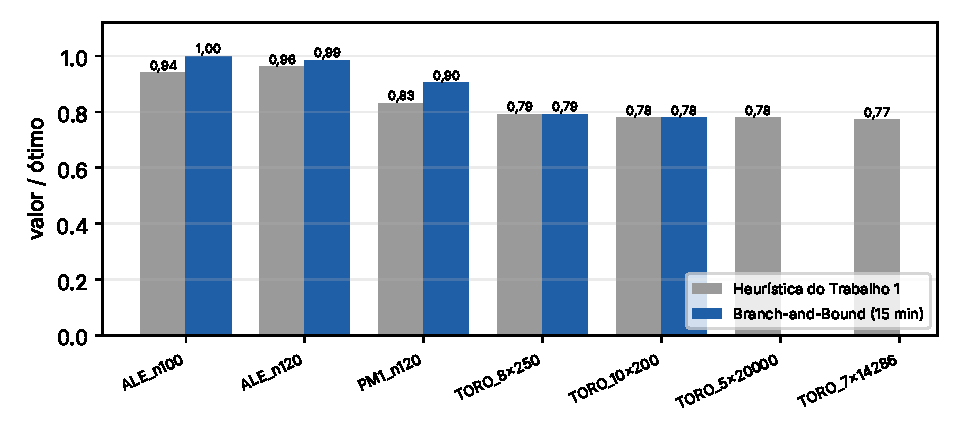
\includegraphics[width=0.92\textwidth]{fig_razao.pdf}
\caption{Valor obtido em relação ao ótimo nas instâncias em que a programação dinâmica calculou o ótimo: heurística do Trabalho~1 (cinza) e Branch-and-Bound com 15 minutos (azul). O Branch-and-Bound não roda nas instâncias de 100 mil vértices.}\label{fig:razao}
\end{figure}

\begin{figure}[ht]
\centering
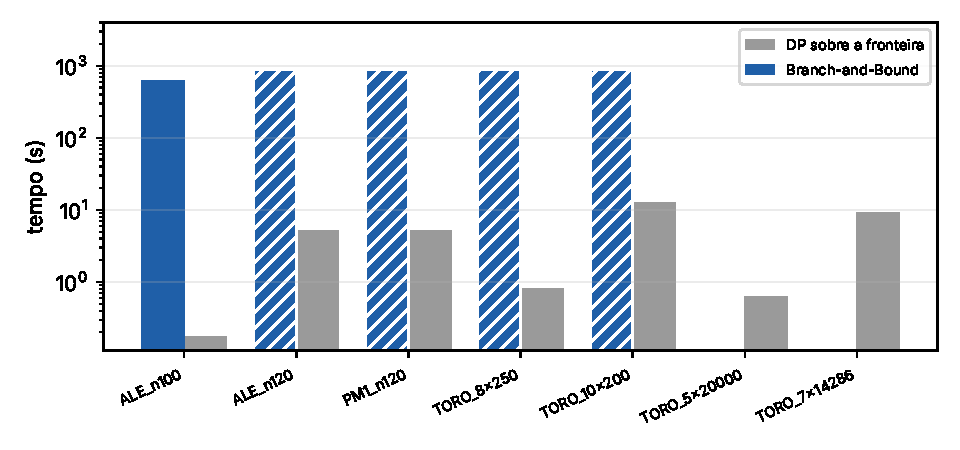
\includegraphics[width=0.92\textwidth]{fig_tempos.pdf}
\caption{Tempo do Branch-and-Bound (azul) e da programação dinâmica (cinza), em escala logarítmica. As barras hachuradas indicam que o Branch-and-Bound parou no limite de 900\,s sem provar o ótimo.}\label{fig:tempos}
\end{figure}

\subsection{Programação dinâmica}

A programação dinâmica calculou o ótimo das 7 instâncias dos grupos A e B, inclusive as duas grades de cerca de 100 mil vértices, em 0,63\,s ($w=11$) e 9,2\,s ($w=15$). O tempo é determinado por $w$ e muito pouco por $n$: nas grades, ele fica em cerca de $3\cdot10^{-9}$\,s por vértice e por estado ($0{,}81$\,s para $n=2\,000$ e $w=17$; $12{,}9$\,s para $n=2\,000$ e $w=21$; $0{,}63$\,s para $n=100\,000$ e $w=11$; $9{,}2$\,s para $n\approx100\,000$ e $w=15$), e a cada 4 bits a mais de largura o tempo se multiplica por cerca de 16, como previsto por $O(n\,2^{w})$. O mesmo vale entre as instâncias 01 e 02 (de $w=21$ para $w=26$ o tempo vai de 0,17\,s para 5,1\,s, um fator de cerca de 30, próximo de $2^5$). A memória acompanha: 12\,MB para $w=11$ e 100 mil vértices, 195\,MB para $w=15$ e 100 mil vértices, 265\,MB para $w=21$ e 2\,000 vértices, e 845\,MB para $w=26$ (limite da implementação). Nas instâncias do grupo C, a ordem encontrada tem fronteira de 41 ou mais, e a programação dinâmica não executa.

\subsection{Branch-and-Bound}

O Branch-and-Bound provou a otimalidade de uma única instância, a \texttt{01\_ALE\_n100} (ótimo 168), depois de 620\,s e $1{,}9\cdot10^{10}$ nós, enquanto a programação dinâmica leva 0,17\,s na mesma instância, cerca de 3\,600 vezes menos. Nas outras 9 instâncias ele chegou ao limite de 900\,s, tendo visitado entre $3{,}1$ e $5{,}2\cdot10^{10}$ nós, a uma taxa de 34 a 57 milhões de nós por segundo (a taxa é maior nas instâncias mais esparsas, onde cada nó custa menos). Esses números enormes são irrelevantes diante do tamanho do espaço de busca ($2^{120}$ em $n=120$, $2^{2000}$ no G32): o tempo gasto não se traduz em prova de otimalidade.

A razão é o limitante \eqref{eq:ub}. A coluna UB/final da Tabela~\ref{tab:bb} mostra que, já na raiz, o limitante fica 18 a 19\% acima do valor final nas instâncias aleatórias com pesos $+1$ pequenas, e entre 24 e 88\% acima nas demais. Nas instâncias com pesos $+1$ a raiz vale exatamente $m$ (200, 240, 400), isto é, o limitante supõe que todas as arestas podem ser cortadas, enquanto o ótimo corta 168 de 200 (84\%) na \texttt{01} e 204 de 240 (85\%) na \texttt{02}. Nas grades, em que metade das arestas tem peso negativo, o limitante da raiz é 2001 contra um ótimo de 1406 (instância 04) e 1386 (05). Um limitante tão folgado só começa a podar quando as arestas já decididas esgotam a folga, e isso demora a acontecer.

Quanto à qualidade da solução devolvida (Figura~\ref{fig:razao}), o Branch-and-Bound melhorou a heurística do Trabalho~1 em 5 das 10 instâncias em que roda e não a melhorou nas outras 5. Nas instâncias aleatórias pequenas ele chegou perto do ótimo: 168 de 168 na \texttt{01} (a heurística tinha 158), 201 de 204 na \texttt{02} (heurística 196) e 75 de 83 na \texttt{03} (heurística 69). Nas grades de 2\,000 vértices (04 e 05) não houve nenhuma melhoria em 15 minutos: o valor final é o da heurística (1\,114 e 1\,080), muito abaixo do ótimo (1\,406 e 1\,386); a busca em profundidade, partindo da solução da heurística, fica presa em uma região do espaço que o limitante não consegue podar. Nas instâncias do grupo C, em que o ótimo não é conhecido, ele melhorou a \texttt{08} (de 316 para 322, $+1{,}9\%$) e a \texttt{10} (de 516 para 528, $+2{,}3\%$), e não alterou a \texttt{09}, o G32 e o G57. Como o limitante da raiz fica de 70 a 73\% acima desses valores, não é possível dizer se a heurística é ótima ou não nessas três instâncias. Isso é o que um Branch-and-Bound com limitante tão fraco pode dar: uma solução e nenhuma garantia.

\subsection{Comparação com o Trabalho 1}

Com os ótimos em mãos, podemos medir a heurística do Trabalho~1 contra o valor verdadeiro (Tabela~\ref{tab:principal} e Figura~\ref{fig:razao}). Nas grades toroidais ela obtém de 77 a 79\% do ótimo (0,792 na \texttt{8x250}, 0,779 na \texttt{10x200}, 0,778 na \texttt{5x20000}, 0,772 na \texttt{7x14286}), e a razão não piora com o tamanho: com 100 mil vértices ela é praticamente a mesma que com 2\,000. Nas aleatórias esparsas com pesos $+1$, 0,94 e 0,96, na faixa de 93 a 96\% do Trabalho~1; com pesos $\pm1$ ela cai para 0,83 (\texttt{03}). Esses números têm a mesma ordem de grandeza dos 80 a 82\% do melhor valor conhecido que o Trabalho~1 relatou nos toroidais do G-set, o que sugere que a diferença se deve sobretudo à busca local 1-flip, que fica presa em ótimos locais ruins, e não a uma referência frouxa. Não podemos dizer o mesmo com certeza para o G32 e o G57: a versão da heurística incorporada ao programa novo dá 1\,170 e 2\,924 (0,83 e 0,84 do melhor valor conhecido, 1\,410 e 3\,494), um pouco acima dos 0,82 do relatório anterior, o que mostra que o desempate da ordenação por grau, e não só o algoritmo, move o resultado em 1 a 3\%. O Branch-and-Bound não alterou esses dois valores em 15 minutos.

O preço do ótimo também fica claro. A heurística leva de 8\,$\mu$s (100 vértices) a 12\,ms (100 mil vértices); a programação dinâmica leva de 0,17\,s a 13\,s nas instâncias em que roda; o Branch-and-Bound, 10 minutos para provar uma instância de 100 vértices e mais de 15 minutos nas demais. A heurística é a escolha certa quando o tempo importa, e os algoritmos exatos servem para medir o quanto ela deixa de ganhar. Nas grades, esse quanto é de 21 a 23\% do ótimo.

\subsection{Comparação com a literatura}

Uma comparação direta de tempos com os resolvedores da literatura não é possível: as instâncias da \emph{Biq Mac Library} e os códigos do \emph{Biq Mac} e do \emph{BiqCrunch} não foram usados, e as máquinas são diferentes. O que podemos dizer é qualitativo. O \emph{Biq Mac} resolve qualquer instância com até $n=100$, mesmo densa \cite{Rendl et al. 2010}; nosso Branch-and-Bound simples provou uma instância esparsa de 100 vértices em 10 minutos e não resolveu as de 120, o que é esperado, já que seu limitante é muito mais fraco que o semidefinido. Nossa programação dinâmica resolve grafos aleatórios esparsos até $n=120$ em 5\,s, mas só porque eles são esparsos; em grafos densos ela seria inviável. Os métodos de branch-and-cut de \citet{Liers et al. 2003} chegam a 1\,280 vértices em grafos aleatórios regulares de grau 4, uma ordem de grandeza acima do que alcançamos em grafos desse tipo (a \texttt{08\_ALE\_n200} está fora do alcance da nossa programação dinâmica, com $w=42$); nossas grades de 100 mil vértices dependem de a largura ser pequena, e não de o algoritmo ser mais forte. Por isso o G-set do Trabalho~1 continua fora do nosso alcance (Tabela~\ref{tab:largT1}).

\subsection{Limitações}

(i) Cada instância foi executada uma vez, em uma única máquina; o limite de 900\,s é arbitrário, e com mais tempo o Branch-and-Bound poderia provar mais uma ou outra instância pequena (a \texttt{01} levou 620\,s). (ii) São 12 instâncias com uma semente cada, o que dá uma boa ideia do comportamento, mas não uma estatística; por exemplo, as razões da heurística em grafos aleatórios pequenos variam bastante entre sementes. (iii) A ordem da programação dinâmica é heurística; uma ordem melhor poderia resolver instâncias maiores, e para as instâncias do grupo C só estimamos a largura com poucas tentativas. (iv) Não foram testadas instâncias de outras fontes (\emph{Biq Mac Library}, outros G-set menores). (v) Nas instâncias 08 a 12, o ótimo é desconhecido, e o valor final do Branch-and-Bound é só um limite inferior.

\section{Conclusão}

Implementamos e validamos dois algoritmos exatos para o Corte Máximo, um Branch-and-Bound com limitante superior incremental e uma programação dinâmica sobre a fronteira de uma ordem dos vértices, ambos com prova de correção e análise de complexidade. Em 12 instâncias de 100 a 100\,002 vértices, com limite de 15 minutos por algoritmo, a programação dinâmica calculou o ótimo de 7 delas, incluindo duas grades toroidais de cerca de 100 mil vértices (em 0,63\,s e 9,2\,s), porque a largura da fronteira é pequena; o tempo cresce com $2^{w}$ e quase não depende de $n$. O Branch-and-Bound provou a otimalidade de uma instância (100 vértices, 620\,s) e esgotou o tempo nas demais, depois de mais de $3\cdot10^{10}$ nós, porque o limitante da raiz fica de 18 a 88\% acima do valor final (Tabela~\ref{tab:bb}). Ainda assim, devolveu soluções melhores que as da heurística em 5 das 10 instâncias em que roda.

Com os ótimos, confirmamos o diagnóstico do Trabalho~1: a heurística gulosa com busca local obtém de 77 a 79\% do ótimo nas grades toroidais com pesos $\pm1$, de 2\,000 a 100 mil vértices, e de 83 a 96\% em grafos aleatórios esparsos pequenos, o que sugere que a diferença em relação ao melhor valor conhecido vem da busca local 1-flip e não de uma referência frouxa. As instâncias do G-set (G32 e G57) continuam fora do alcance dos dois algoritmos: a programação dinâmica exigiria fronteira de 41 ou mais, e o Branch-and-Bound não melhorou a heurística em 15 minutos.

Como trabalho futuro, o ganho mais claro está em limitantes melhores para o Branch-and-Bound, por exemplo com empacotamento de ciclos ímpares ou relaxações lineares e semidefinidas, que é o que a literatura usa para instâncias desse porte; e em ordens melhores para a programação dinâmica, ou no uso de decomposições em árvore. Por fim, valeria rodar os algoritmos nas instâncias da \emph{Biq Mac Library} para uma comparação direta de tempos com a literatura.
